\section{Instalações industriais, QGBT, CCM e motores}

\begin{frame}{Arquitetura industrial típica}
\small
\centering
\begin{tikzpicture}[scale=0.83,every node/.style={font=\scriptsize}]
\tikzset{b/.style={draw=corPrim,fill=corDef!7,rounded corners,minimum width=2.45cm,minimum height=0.67cm,align=center}}
\node[b] (mt) at (0,3.2) {Rede MT};
\node[b] (sub) at (0,2.2) {Subestação / trafo};
\node[b] (qgbt) at (0,1.2) {QGBT};
\node[b] (ccm) at (-3.4,0.0) {CCM / motores};
\node[b] (qd) at (0,0.0) {QD / processo};
\node[b] (ups) at (3.4,0.0) {UPS / críticas};
\node[b] (m) at (-3.4,-1.2) {Bombas / ventiladores};
\node[b] (p) at (0,-1.2) {Força / iluminação};
\node[b] (clp) at (3.4,-1.2) {CLP / TI / instrumentos};
\foreach \u/\v in {mt/sub,sub/qgbt,qgbt/ccm,qgbt/qd,qgbt/ups,ccm/m,qd/p,ups/clp}{\draw[-{Stealth},thick,corPrim] (\u)--(\v);}
\end{tikzpicture}
\vspace{2mm}
\begin{caixaObs}
Na indústria, a decisão técnica precisa incluir disponibilidade, manutenção, expansão e custo da parada de processo.
\end{caixaObs}
\end{frame}

\begin{frame}{QGBT: especificação técnica}
\small
\begin{columns}[T,onlytextwidth]
\column{0.52\textwidth}
\begin{itemize}
\item Tensão e corrente nominal do conjunto.
\item Corrente de curto suportável e barramentos.
\item Grau de proteção e condições ambientais.
\item Segregação/compartimentação conforme necessidade.
\item Dissipação térmica e ventilação.
\item Medição, supervisão, comunicação e reservas.
\end{itemize}
\column{0.46\textwidth}
\begin{caixaNorma}[title=Série NBR IEC 61439]
O quadro deve ser tratado como \textbf{conjunto}, com responsabilidades de projeto/montagem e verificações aplicáveis -- não como simples reunião de dispositivos individuais certificados.
\end{caixaNorma}
\begin{caixaAt}
Icc do dispositivo não substitui a análise da suportabilidade do conjunto e dos barramentos.
\end{caixaAt}
\end{columns}
\end{frame}

\begin{frame}{CCM: centro de controle de motores}
\small
\begin{columns}[T,onlytextwidth]
\column{0.49\textwidth}
\begin{itemize}
\item Alimentação e distribuição para motores.
\item Proteção, seccionamento e manobra.
\item Partida direta, soft-starter, inversor.
\item Relés eletrônicos e monitoramento.
\item Interface com CLP, IHM e supervisório.
\item Intertravamentos e segurança operacional.
\end{itemize}
\column{0.49\textwidth}
\centering
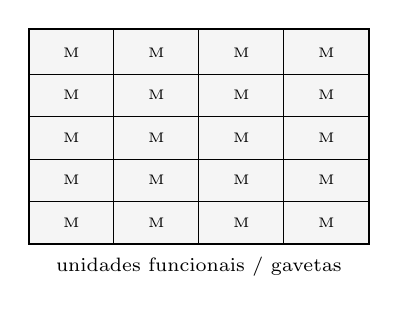
\begin{tikzpicture}[scale=0.72,every node/.style={font=\tiny}]
\draw[thick,fill=black!4] (0,0) rectangle (6.0,3.8);
\foreach \x in {1.5,3.0,4.5}{\draw (\x,0)--(\x,3.8);}
\foreach \y in {0.75,1.5,2.25,3.0}{\draw (0,\y)--(6.0,\y);}
\foreach \x in {0.75,2.25,3.75,5.25}{\foreach \y in {0.38,1.13,1.88,2.63,3.38}{\node at (\x,\y){M};}}
\node[font=\scriptsize] at (3.0,-0.4) {unidades funcionais / gavetas};
\end{tikzpicture}
\end{columns}
\end{frame}

\begin{frame}{Motor de indução: corrente e partida}
\small
\begin{columns}[T,onlytextwidth]
\column{0.51\textwidth}
\begin{align*}
I_N&=\frac{P_{out}}{\sqrt3V\eta fp}\\
I_{part}&\approx k_p I_N
\end{align*}
\begin{itemize}
\item $k_p$ depende do motor e método de partida.
\item Partida afeta queda de tensão e dimensionamento da rede.
\item Proteção precisa considerar sobrecarga, curto, falta de fase e travamento.
\end{itemize}
\column{0.47\textwidth}
\begin{tikzpicture}
\begin{axis}[width=5.7cm,height=3.9cm,xlabel={tempo},ylabel={$I/I_N$},xmin=0,xmax=6,ymin=0,ymax=7,grid=both,legend pos=north east]
\addplot[corPrim,thick] coordinates {(0,6.2)(0.5,5.8)(1,4.5)(2,2.2)(3,1.2)(6,1)};\addlegendentry{direta}
\addplot[corAccent,thick,dashed] coordinates {(0,2.8)(0.5,2.5)(1,2)(2,1.4)(3,1.05)(6,1)};\addlegendentry{rampa}
\end{axis}
\end{tikzpicture}
\end{columns}
\end{frame}

\begin{frame}{Comparação de métodos de partida}
\scriptsize
\begin{tabularx}{\textwidth}{>{\bfseries}p{2.5cm}p{2.7cm}p{2.8cm}X}
\toprule
Método & Corrente de partida & Torque/controle & Quando faz sentido \\
\midrule
Direta & Alta & Torque natural do motor & Rede robusta, motor pequeno/médio e processo tolerante. \\
Estrela-triângulo & Reduzida & Torque também reduzido & Motor compatível e carga que acelera com torque reduzido. \\
Soft-starter & Rampa de tensão & Partida/parada suave & Bombas, ventiladores e redução de impacto mecânico/hidráulico. \\
Inversor & Controlada & Velocidade e torque variáveis & Processo exige controle, economia e flexibilidade. \\
\bottomrule
\end{tabularx}
\vspace{2mm}
\begin{caixaAt}
Não escolher pelo preço do equipamento isoladamente: comparar rede, carga mecânica, ciclo, eficiência, harmônicas, manutenção e controle.
\end{caixaAt}
\end{frame}

\begin{frame}{Inversor de frequência: efeitos na instalação}
\small
\begin{columns}[T,onlytextwidth]
\column{0.51\textwidth}
\begin{itemize}
\item Retificador gera correntes não senoidais na entrada.
\item PWM na saída cria alto $dv/dt$ e correntes de modo comum.
\item Comprimento do cabo ao motor pode exigir filtro/reator.
\item Blindagem e aterramento afetam EMC.
\item Correntes de fuga interferem na escolha do DR.
\end{itemize}
\column{0.47\textwidth}
\centering
\begin{tikzpicture}[every node/.style={font=\scriptsize}]
\tikzset{b/.style={draw=corPrim,fill=corDef!7,rounded corners,minimum width=2.2cm,minimum height=0.58cm}}
\node[b] (rede) at (0,4.4) {Rede CA};
\node[b] (ret) at (0,3.3) {Retificador};
\node[b] (dc) at (0,2.2) {Link CC};
\node[b] (inv) at (0,1.1) {PWM};
\node[b] (mot) at (0,0) {Motor};
\foreach \u/\v in {rede/ret,ret/dc,dc/inv,inv/mot}{\draw[-{Stealth},thick,corPrim] (\u)--(\v);}
\draw[corNorma,thick] (mot.south)--(0,-0.8) node[ground]{};
\end{tikzpicture}
\end{columns}
\end{frame}

%=====================================================================
